%!TeX root=./maximo.tex

\section{Heap Cinético}
\label{heap:secao}
Um bom jeito de resolver o problema do máximo cinético é manter uma
fila de prioridades com os elementos da coleção tendo como
prioridade o valor corrente do elemento. Dessa maneira, o elemento
que se encontra na raiz da fila será o que possui o maior valor da
coleção. Para implementar a fila utilizaremos um vetor organizado
como um heap.

Inicialmente o vetor começa com os índices dos elementos e
reorganizamos como um heap usando como chave o valor de cada
elemento no instante $t = 0$, ou seja, o valor $x_0$ de cada
elemento.

Uma vez montado o heap, construímos um certificado para cada par
$($filho, pai$)$ no heap. O $i$-ésimo certificado, que se refere ao
par das posições $i$ e $\floor{\frac{i}{2}}$, consiste no instante
de tempo em que o $i$-ésimo elemento passará a ter um valor maior
que o valor do $\floor{\frac{i}{2}}$-ésimo elemento do vetor, se
esse instante for maior que o instante atual. Do contrário, o
certificado consiste em $+\infty$.

Esses $n - 1$ certificados são colocados em uma fila com prioridades
$Q$, com o prazo de validade como chave. Estamos interessados nos
certificados com menor prazo de validade.

Para descrever a implementação das três operações, precisamos
estabelecer o nome das novas variáveis usadas. São elas:
\begin{enumerate}
    \item \textit{heap}: vetor com os índices dos $n$ elementos
    formando um heap de acordo com o seu valor no instante
    \textit{now};
    \item \textit{cert}: vetor com os certificados, onde
    \textit{cert}$[i]$ guarda o certificado entre $i$ e
    $\floor{\frac{i}{2}}$, para $1 < i \leq n$.
\end{enumerate}

A interface da fila com prioridades que utilizaremos não se altera.

Um evento está associado a um certificado $(i, t)$ que expira no
instante $t$, como pode ser visto na Figura \ref{fig:maxdevent}. O
tratamento do evento correspondente ao certificado $(i, t)$ consiste
em trocar de lugar os índices armazenados nas posições $i$ e
$\floor{\frac{i}{2}}$ do vetor \heap, e recalcular o prazo de
validade de até cinco certificados, ilustrados na Figura
\ref{fig:max:update}:
\begin{itemize}
    \item do $\floor{\frac{i}{2}}$-ésimo certificado, se $i > 1$;
    \item do $j$-ésimo certificado, se $i > 1$ e $j \leq n$,
    onde $j = 2\cdot \floor{\frac{i}{2}} + ((i + 1)\mod2)$
    é o irmão de $i$;
    \item do $(2i)$-ésimo certificado, se $2i \leq n$;
    \item do $(2i + 1)$-ésimo certificado, se $2i + 1 \leq n$.
\end{itemize}

\begin{figure}[H]
    \centering
    \RawFloats
    \begin{minipage}{.5\textwidth}
        \centering
        \begin{figure}[H]
    \centering
    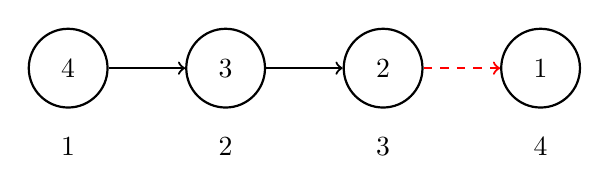
\begin{tikzpicture}[thick]
        \edef\pos{0}
        \foreach \x in {1, 2,..., 4}{
            \pgfmathparse{\pos+2}
            \xdef\pos{\pgfmathresult}
            \node  at (\pos, -1) {$\x$};
        }
        \node[circle,draw, minimum size=1cm] (1) at  (2, 0) {$4$};
        \node[circle,draw, minimum size=1cm] (2) at  (4, 0) {$3$};
        \node[circle,draw, minimum size=1cm] (3) at  (6, 0) {$2$};
        \node[circle,draw, minimum size=1cm] (4) at  (8, 0) {$1$};
        \draw[->] (1) -- (2);
        \draw[->] (2) -- (3);
        \draw[->, color=red, dashed] (3) -- (4);
    \end{tikzpicture}
    \caption[Exemplo de expiração de certificado da lista ordenada]{No exemplo da
    Figura~\ref{fig:ordenacao:exemplo}, \cert[3] expirou no instante $t = 2$.}
    \label{fig:lista:expire}
\end{figure}
        \caption[Certificado expirado]{\cert[$4$] expirou.}
        \label{fig:maxdevent}
        \vspace{\baselineskip}
        \vspace{\baselineskip}
    \end{minipage}%
    \begin{minipage}{.5\textwidth}
        \centering
        \begin{algorithm}[H]
    \caption{Função \textsc{update}.} \label{torneioi:update}
    \begin{algorithmic}[1]
        \Function{update}{$e$}
            \If{$e \neq$ NULL}
                \State $e'\leftarrow \torneio[(e.\lastmatch)/2]$
                \State $t \leftarrow $ \Call{expire}{$e, e'$}
                \State \Call{updatePQ}{$Q,e,t$}
            \EndIf
        \EndFunction
        % \LineComment{Em expire$(e, e')$, $e'$ pode ser nulo e
        % nesse caso o retorno é $+\infty$.}
        % \LineComment{\Call{expire}{$e,e'$} calcula a validade do
        % certificado entre os elementos $e$ e $e'$, se $e'$ é NULL
        % retorna $+\infty$}
    \end{algorithmic}
\end{algorithm}
        \caption[Exemplo de atualização de certificados no heap cinético]{\heap[$4$] e \heap[$2$]
        foram trocados e \cert[$2$], \cert[$4$], \cert[$5$],
            \cert[$8$] e \cert[$9$] foram atualizados.}
        \label{fig:max:update}
    \end{minipage}
\end{figure}

O $i$-ésimo certificado também deve ser ajustado para $+\infty$.
Finalmente, é necessário fazer ajustes em $Q$, alterando a chave dos
certificados que sofreram alteração.

Novamente, na implementação da operação \textsc{event}, no Algoritmo
\ref{max:evento}, utilizaremos a rotina \textsc{update}$(i)$, do
Algoritmo \ref{max:update}, que calcula a nova validade $t$ do
$i$-ésimo certificado, se $1 < i \leq n$, e chama a rotina
\textsc{updatePQ}$(Q, i, t)$.

\begin{algorithm}[H]
    \caption{Função \textsc{update}.} \label{torneioi:update}
    \begin{algorithmic}[1]
        \Function{update}{$e$}
            \If{$e \neq$ NULL}
                \State $e'\leftarrow \torneio[(e.\lastmatch)/2]$
                \State $t \leftarrow $ \Call{expire}{$e, e'$}
                \State \Call{updatePQ}{$Q,e,t$}
            \EndIf
        \EndFunction
        % \LineComment{Em expire$(e, e')$, $e'$ pode ser nulo e
        % nesse caso o retorno é $+\infty$.}
        % \LineComment{\Call{expire}{$e,e'$} calcula a validade do
        % certificado entre os elementos $e$ e $e'$, se $e'$ é NULL
        % retorna $+\infty$}
    \end{algorithmic}
\end{algorithm}

\begin{algorithm}[H]
    \caption{Função \textsc{event}.} \label{torneioi:evento}
    \begin{algorithmic}[1]
        \Function{event}{\nnull}
            \State $e \leftarrow  $ \Call{minPQ}{$Q$}
            \While{$e.\cert$ = \now}
                \State $j \leftarrow e.\lastmatch$
                \State $k \leftarrow 2\cdot \floor{\frac{j}{2}}
                + ((j + 1)\mod2)$ \Comment{adversário}
                \While{$j > 1$ \AND \Call{value}{$j$} $\geq$
                    \Call{value}{$k$}}
                    \State \torneio[$\floor{\frac{j}{2}}$]
                    $\leftarrow~$\torneio[$j$]
                    \State $\torneio[k].\lastmatch$ $\leftarrow k$
                    \State \Call{update}{$\torneio[k]$}
                    \State $j \leftarrow \floor{\frac{j}{2}}$
                    \State $k \leftarrow 2\cdot \floor{\frac{j}{2}}
                    + ((j + 1)\mod2)$ \Comment{adversário}
                \EndWhile
                \State $\torneio[j].\lastmatch \leftarrow j$
                \State \Call{update}{$\torneio[j]$}
                \State $e \leftarrow  $ \Call{minPQ}{$Q$}
            \EndWhile
        % \LineComment{swapHeap$(i, \floor{\frac{i}{2}})$ troca \heap[$i$] por \heap$\left[\floor{\frac{i}{2}}\right]$}
        \EndFunction
%        \LineComment{\Call{compare}{$i, j$} retorna se o valor
%        de $i$ é maior que o valor de $j$.}
    \end{algorithmic}
\end{algorithm}

A operação \textsc{query\_max}$()$, no Algoritmo
\ref{max:heap:querymax}, consiste em devolver \textit{heap}$[1]$,
enquanto que a operação \textsc{change}$(j, v)$, no Algoritmo
\ref{max:heap:change}, consiste em alterar a posição $x_0[j]$ para
${x_0[j] + (\mathit{speed}[j] - v)\cdot now}$, a posição
\textit{speed}[j] para \textit{v} e recalcular os eventuais
certificados de que $j$ participa. Para tanto, a partir da posição
$i$ em que $j$ se encontra no vetor \textit{heap}, podemos
recalcular \textit{cert}$[i]$ se $i > 1$, \textit{cert}$[2i]$ se $2i
\leq n$ e \textit{cert}$[2i + 1]$ se $2i + 1 \leq n$, acionando a
rotina \textsc{update} para fazer os devidos acertos em $Q$
correspondentes a estas modificações. Veja a Figura
\ref{fig:predeventheap}.

\begin{algorithm}
    \caption{Função \textsc{query\_max}.} \label{torn:querymax}
    \begin{algorithmic}[1]
        \Function{query\_max}{\nnull}
            \State \Return \torneio$[1]$
        \EndFunction
    \end{algorithmic}
\end{algorithm}

\begin{algorithm}
    \caption{Função \textsc{change}.} \label{lista:change}
\begin{algorithmic}[1]
    \Function{change}{$j, v$}
        \State $x_0$[$j$] $\leftarrow  x_0$[$j$]
        $+~($\speed[$j$]$~-~v)~\cdot~$\now;
        \State \speed[$j$] $\leftarrow  v$
        \State $i \leftarrow$ \inds[$j$]
        \State \Call{update}{$i$}
        \State \Call{update}{$i - 1$}
    \EndFunction
\end{algorithmic}
\end{algorithm}

\begin{figure}
    \centering
    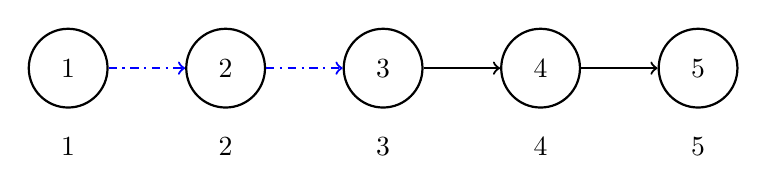
\begin{tikzpicture}[thick]
        \edef\pos{0}
        \foreach \x in {1, 2,..., 5}{
            \pgfmathparse{\pos+2}
            \xdef\pos{\pgfmathresult}
            \node[circle,draw, minimum size=1cm] (\x) at
                (\pos, 0) {$\x$};
            \node  at (\pos, -1) {$\x$};
        }
        % \foreach \x [evaluate=\x as \y using int(\x + 1)] in {1, 2,..., 4}{
        %     \ifthenelse{\x==2}{\draw[->, draw=red] (\x) -- (\y);}{\draw[->, draw=black] (\x) -- (\y);}
        % }
        \draw[->, color=blue, dashdotted] (1) -- (2);
        \draw[->, color=blue, dashdotted] (2) -- (3);
        \draw[->] (3) -- (4);
        \draw[->] (4) -- (5);
        % \draw[->] (1) edge (2) (2) edge (3) (3) edge (4) (4) edge (5)
    \end{tikzpicture}
    \caption[Certificados atualizados]{Após a mudança de velocidade
            do elemento 2, que se encontra em \sorted[2], \cert[1] e
            \cert[2] foram atualizados.}
    \label{fig:lista:after}
\end{figure}
